

The first goal of the proposed work is to further develop the Fusion browser extension prototype described in \Cref{chap:fusion} for a public field deployment and test the system at scale and in real-life scenarios. Based on lab studies and interviews with the participants, I have identified two areas of user needs that are critical and currently not supported by the system. More specifically, many participants expressed the need to save and manage many information sources (i.e., entire webpages instead of short clips) for different purposes, citing how conducting complex search tasks can lead to an overwhelming amount of opened tabs that can be difficult to manage.
Participants also pointed to the limitation of saving notes to entity cards generated by the system, and wanted to organize information more flexibly to reflect their evolving mental models throughout the process. Addressing these has the potential of allowing the system to better supporting the next steps in online sensemaking -- structuring collected information while efficiently managing multiple information sources.

My primary focus will be on further developing the research prototype for a public release while experimenting with new approaches within the same system to support structuring and source (webpages) management. While a public deployment has the potential of allowing the system to reach a wider audience outside of the lab and collect usage information at scale, user tests and lab studies may also be required throughout the process of system design and development.
Success in gaining popularity would also depend on many factors outside of the scope of my dissertation, such includes visual design, marketing and market understanding, and competing commercial products. While the aim is to develop a large user-base, the proposed approaches can also be evaluated with lab studies and smaller scale field deployments using participants recruited from a local participant pool (CBDR). 




\section{Preliminary Study: Challenges in Tabbed Browsing Behavior}

\begin{table*}
\centering
\footnotesize
  \def\arraystretch{1.1}
  
  \begin{tabular}{l p{11.6cm}}
  
  \hline
  \multicolumn{2}{c}{Different Pressures for Closing Tabs versus Keeping Tabs Opened} \\
  \hline
  
    \textbf{C1}.Limited Attention &
    Keeping too many tabs can be overwhelming and makes it difficult to focus \\
    
    \textbf{C2}.Screen Real-estate &
    Having too many tabs makes it hard to navigate and have situational awareness \\
    
    \textbf{C3}.Computing power &
    Drains processors and memory, causing browser and other applications to slow \\
    
    \textbf{C4}.To be Organized &
    Social and self pressure to avoid looking disorganized \\
    
    \hline
    
    \textbf{O1}.Remind and Resume &
    Keeping tabs around as a reminder to work on them or keep track of progress \\

    \textbf{O2}.Revisit References &
    Keeping frequently used tabs for quick access; has a diminishing return \\
    
    \textbf{O3}.Costly Re-finding &
    Avoid closing tabs in fear of not being able to re-find valuable information \\
    
    \textbf{O4}.Aspiration/Sunk Cost  &
    The hopes to process more information than capable; while aware of the situation \\
    
    \textbf{O5}.Mental Model &
    Tabs and windows represent external memory and mental models for complex tasks \\
    
    \textbf{O6}.Uncertain Relevance &
    Difficulties in judging the current and potential relevance of tabs in the future \\
    
    \hline

  \end{tabular}

  \caption[An overview of our findings in the tab usage study.]{Browser tabs are overloaded with different functionalities, such as todo items, external memory, or references, leading to two sets of opposing pressures that drive tabbed browsing behavior.}
  \label{tab:tabs_overview}
\end{table*}

Browser tabs have become an integral part of how people browse and navigate the web since they were introduced in the early 2000s, and have since became an ubiquitous feature in all major web browsers. However, since their introduction, the internet has gone through dramatic changes. Tabs are now simultaneously used to check emails, control media players, stash articles to read later, organize references, plan trips, research products, write articles. More fundamentally, online information seeking has evolved from navigating web directories to find useful websites (e.g. DMOZ \cite{dmoz}) to searching the entire web for dozens to hundreds of individual webpages to support complex sensemaking tasks \cite{pirolli1999information,marchionini2006exploratory}. These changes reflect an increasing amount of dependence on the functionality and interfaces of modern web browsers in meeting these needs.
Despite this expansion of functionality, browser tabs still remain instantiated as simple temporally-ordered lists with few contextual cues. 
There is increasing evidence that using tabs for this wide array of functions leads to breakdowns, overload, and missed opportunities \cite{web1, web2, web3, web4, web5}.
%Indeed, the fixation on tabs as a metaphor is so strong that the most popular changes to using tabs involve relatively small design adjustments such as making them a vertical instead of horizontal list \cite{vtabs} or creating tabs that contain more tabs \cite{treetabs}. 

To investigate design opportunities that can expand the current prototype to better support the process of searching, foraging, and structuring, I conducted an empirical study on the challenges people face when using modern browsers. Instead of examining the specific functions of tabs as they are currently used (e.g., as in Dubroy, 2010 \cite{Dubroy:2010:STB:1753326.1753426}), I focus on developing a model of the way that tabs break down from their daily use. 
Ten graduate strudents or full-time researchers were recruited from the university and a research facility as participants for in-person interviews (age: M=23.0, SD=4.7, min=19, max=32, 40\% male).
Participants were first asked to walk through each tab they had opened on their work computers and explain the tasks, goals, or purposes of why each tab was opened in the first place and why it was kept opened, using questions including ``\emph{Was this tab intentionally kept around for later usage?}'' If answered ``\emph{yes}'', we followed up with ``\emph{Did you came back to it recently, why or why not?}'' And if answered ``\emph{no}'', we followed up with ``\emph{Why was this tab kept around if you did not plan to use it again?}'', and ``\emph{Do you struggle to close your tabs?}''  We also asked about how and how effective are they managing their tabs with questions include ``\emph{How frequently do you evaluate your tabs to see if you can close them? How difficult is it?}'', and ``\emph{Does the number of tabs you have opened affect how you feel?}'' The interviews were recorded, transcribed, and analyzed using a grounded theory approach with four rounds of discussions and coding \cite{strauss1998basics}.

Table \ref{tab:tabs_overview} shows an overview of major drivers people encountered while using tabs for information work.
Overall, these drivers could be classified as two opposing forces: pressures to close tabs, and pressures to keep tabs open.  I found strong evidence that participants had a number of pressures to close their many tabs, ranging from limited human attention to limited computing resources to self presentation.  At the same time, there are also a diverse set of drivers making it not so simple to close tabs even under these pressures. These included previously reported drivers such as reminding users of unfinished tasks \cite{Dubroy:2010:STB:1753326.1753426}, but also new factors relating to cost structure of tabbed browsing, such as the cost of re-accessing pages, the sunk costs of finding and organizing information, the benefits of supporting an (unrealistic) aspirational self, and the uncertainty of the expected value of information in the future, especially when searching in unfamiliar domains. These pressures to close vs. keep open tabs interact to create feelings of stress, being overwhelmed, and even shamefulness of appearing unorganized in our participants. These findings have implications for the design of new forms of web browsing that can better support the underlying drivers behind the use of tabs. In the next two subsection, I propose two approaches that aim to better support issues caused by different drivers that we characterized from both \Cref{chap:fusion} and this preliminary study.

\begin{figure}
\centering
\begin{minipage}{.49\textwidth}
  \centering
  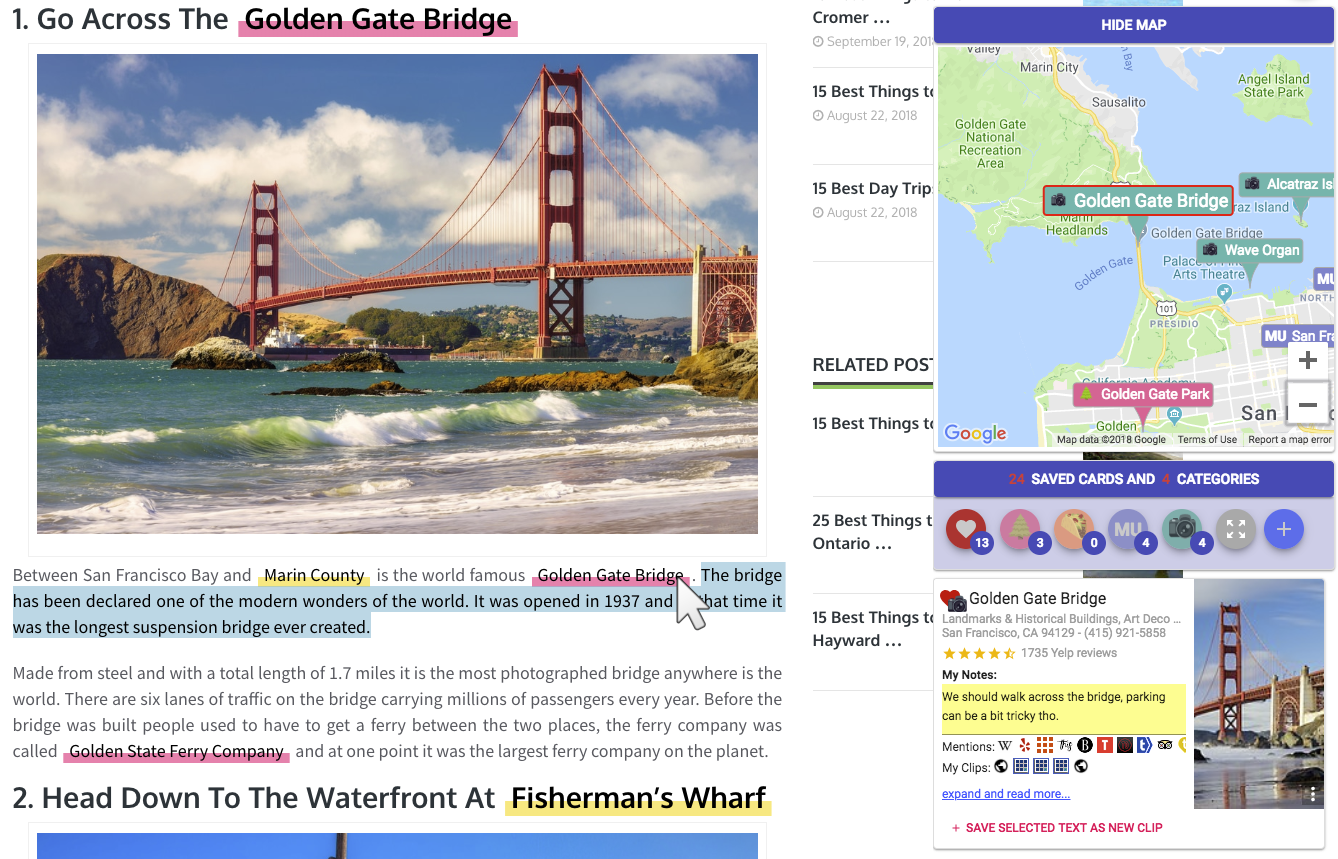
\includegraphics[width=\textwidth]{Chapters/Fusion/main.png}
\end{minipage}%
\begin{minipage}{.49\textwidth}
  \centering
  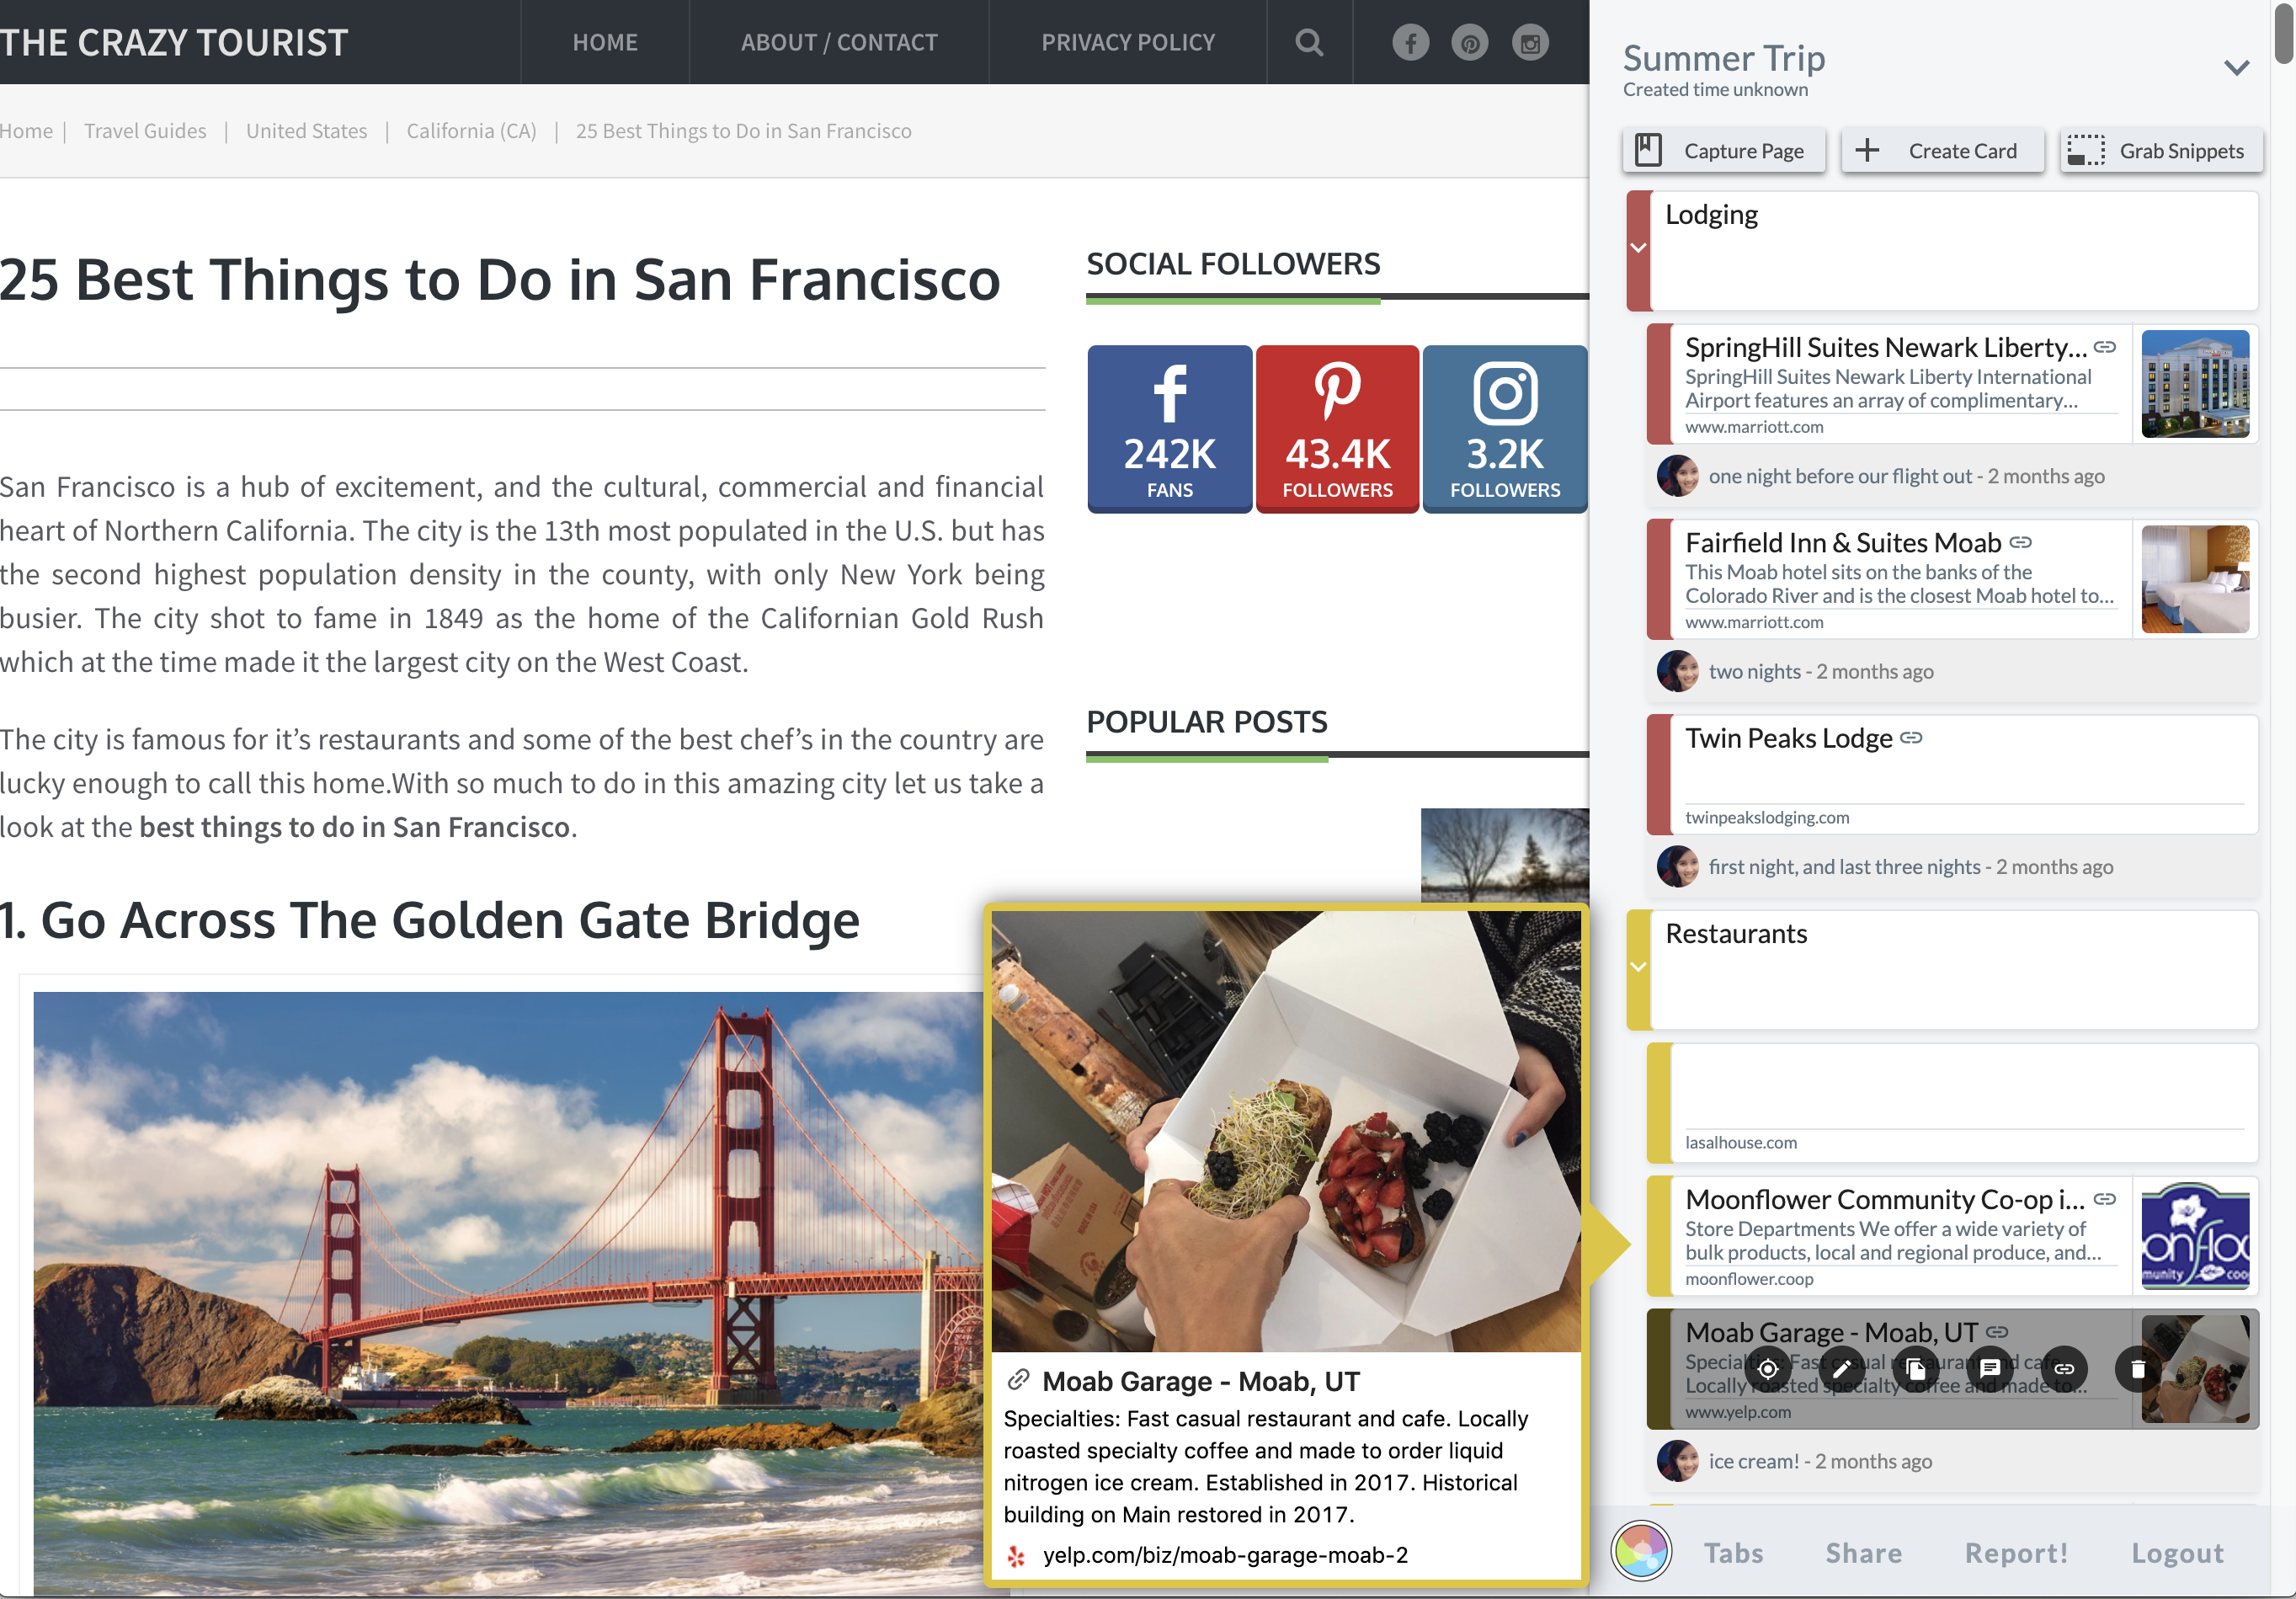
\includegraphics[width=\textwidth]{images/fuse.png}
\end{minipage}
\caption{The current prototype allowed users to access entity cards generated by the system, and saved on into categories (left). In the new design, users can also create notes and category cards, and nest cards to create a hierarchy structure (right).}
\label{fig:test2}
\end{figure}


\section{Foraging and Structuring Information}% (O2, O3, O5)}

In \Cref{chap:fusion} I presented a prototype system called Fusion Browser that focused on exploiting common entities mentioned across webpages in a complex search task as a substrate to support foraging. One the features of Fusion Browser is to allow users to save information about an entity to be propagated and resurfaced across other webpages that also mentioned the same entity, allowing users to efficiently cross-reference and build on their prior effort as they explore more webpages. While participants generally agreed that this entity-centric approach lowered the cost of saving information and accessing them during complex search tasks involving multiple webpages, they also pointed to its limitations. Specifically, the current prototype only allowed users to attach information to entity cards and organize cards under categories. While participants found this to be effective for foraging, they also expressed needs for creating structures more flexible than categories of pre-compiled entity cards that can better reflect their changing mental models. They cited their current practices of using word processors (such as Google Docs) to create outlines or tables containing both information copied from webpages and manual notes about their own thoughts and decisions. In addition, similar to participants from the preliminary study, participants from \Cref{chap:fusion} also reported the need to save links of useful webpages.

Due to its ubiquity and generalizability, I plan to extend the current prototype to support building outlines during foraging. In the new design, instead of attaching collected information to entity cards created by the system, users can freely create manual note cards to externalize their thoughts and decisions. To create structures that can better reflect users' mental models, in the new design users can also nest cards under other cards to create hierarchies. This design is similar to how many participants reported using note taking software during complex search tasks, but the core challenge here is to lower the cost of structuring and externalization as they can be either disruptive for users' reading process or prohibitive for externalizing \cite{o1996towards,marshall1999introducing,tashman2011liquidtext,bianchi2015designing}. My insights from developing Fusion Browser (\Cref{chap:fusion}) that focused on in-situ information foraging represent a unique starting point for investigating ways to support in-situ information structuring as users explore and foraging from multiple webpages in a complex search task. In addition, my past work on the Alloy system (\Cref{chap:alloy}) for structuring web content with machine learning and crowd-microtasks can also provide insights on designs and interactions that can further lower the costs of structuring for the end users through machine learning.

\section{Managing Information Sources in the Browser}% (O1, O4, O6)}

From the preliminary interviews and the lab studies from \Cref{chap:fusion}, We also observed that exploratory searches can lead to large numbers of open tabs in a short period of time, and quickly becomes difficult for the users to manage. These tabs can also be overloaded with different purposes, such as queuing up to-do tasks, reminders for things to go back to, or potential future references. Existing approaches for saving browser tabs have different issues. For example, the built-in bookmarking feature saves tab in a separate folder structure. This not only introduce additional costs of maintaining a structure separated from users notes, but can also create conflicting mental model representations requiring users' cross-refernce between them. In addition, turning a browser tab into a bookmark in the browser also makes it much less accessible and out of sight for the users when compared to tabs. On the other hand, popular bookmarking browser extensions such as OneTab\footnote{\url{https://www.one-tab.com/}} allow users to save and re-open sets of tabs as sessions for resumption retain more task structures, but also takes away many features of browser tabs such as reminding. I plan to extend the current system to provide better support for managing information sources during online sensemaking tasks to address issues introduced by tab overload, such as:

\begin{itemize}
    \item Allowing users to organize information sources using their existing notes outline vs creating a separate bookmark folder structure.
    \item Allowing users to close and save tabs and indicate their current functions. For example, closing tabs and marking them as reminders or to-dos, useful references, or articles a user aspired to read.
    \item The system can in turn use different strategies to resurface previously saved tabs. For example, showing reminder tabs in prominent places such as the default newtab page, resurfacing references when users is reading about a related webpage, or proactively encourage users to read previously saved articles when they were browsing social networks.
\end{itemize}

These designs were informed by the preliminary interviews.

\section{Evaluation and Contributions}

%I plan to conduct studies to explore this idea in two phases: First, a controlled lab study focusing on how this entity-centric approach can benefit foraging across webpages. I will use the findings from study 1 to inform the development and public release of a browser extension that supports both entity-centric foraging and structuring.

%For Study 1, I will build a prototype system for a controlled lab study to explore the benefits and challenges of the entity-centric approach for reading, cross-referencing, and collecting information across multiple webpages in the browser. I plan to explore whether the gather- and propagate-based features can allow participants to cross-reference and re-access previously saved notes efficiently and whether participants consider having the additional features an improvement to their current methods.
Since note taking and structuring are longer term activities when compared to foraging, I plan to publically release a browser extension for Chrome to reach a wider audience, collect usage information. This would allow me to gather quantitative data based on real-life tasks, for example: 

\begin{itemize}
    \item Time spent using the system
    \item Types of tasks conducted
    \item Features utilized
    \item Number of cards and notes created per task
    \item Types of structures created
\end{itemize}

Throughout development, I will also conduct lab studies and usability tests to collect qualitative data and better understand how users may utilize the system, for example:

\begin{itemize}
    \item General usability of the system
    \item Confidence in their process and decisions
    \item Overall preferences, satisfaction and motivation
\end{itemize}

The core contribution of the proposed work is an in-situ and context-aware approach for supporting sensemaking across webpages in the browser when conducting complex exploratory search tasks, which includes:

\begin{itemize}
\item An extension that enables the browser to better understand the content of webpages by identifying entities using existing natural language processing algorithms and external knowledge sources (e.g., Wikipedia and Yelp), lowering the cost of cross-referencing different entities across webpages, searches, and external knowledge sources. 
\item A context-aware workspace where users can easily gather and structure options and evidence across multiple webpages, where relevant information saved previously will be resurfaced by the system as users browse different pages.
\item Qualitative analysis on issues that information workers face when trying to manage multiple browser tabs during complex tasks, and a set of new approaches for managing multiple online sources under uncertainty that aim to address such issues.
\end{itemize}

Equipping browsers and note-taking interfaces the ability to identify and connect options and evidence scattered across tabs and personal notes have the potentials of lowering the efforts required to make sense of and forage from many information sources. Empowering users to capture, associate, and structure fluidly their findings as they read and understand more information. Successes in doing so may also lead to useful insights on the design of future intelligent browser interfaces that can better understand the information being consumed by its users, and building novel interactive systems for supporting online sensemaking.


\section{Timeline and Submission Plans}

\subsection*{Timeline}

\begin{itemize}
    \item April - June 2019: Prototype Development
    \item June - August 2019: Deployment
    \item August - September 2019: Evaluation and Analysis
    \item October - December 2019: Write Dissertation and Defend 
\end{itemize}

\subsection*{Submission Plans}

\begin{itemize}
    \item ACM UIST 2019: \Cref{chap:fusion}
    \item ACM SIGCHI 2019: \Cref{chap:proposed}
\end{itemize}